\documentclass[11pt,a4paper]{report}
\usepackage[textwidth=37em,vmargin=30mm]{geometry}
\usepackage{calc,xunicode,amsmath,amssymb,paralist,enumitem,tabu,booktabs,datetime2,xeCJK,xeCJKfntef,listings}
\usepackage{tocloft,fancyhdr,tcolorbox,xcolor,graphicx,eso-pic,xltxtra,xelatexemoji}

\newcommand{\envyear}[0]{2025}
\newcommand{\envdatestr}[0]{2025-05-10}
\newcommand{\envfinaldir}[0]{webdb/2025/20250510/final}

\usepackage[hidelinks]{hyperref}
\hypersetup{
    colorlinks=false,
    pdfpagemode=FullScreen,
    pdftitle={Web Digest - \envdatestr}
}

\setlength{\cftbeforechapskip}{10pt}
\renewcommand{\cftchapfont}{\rmfamily\bfseries\large\raggedright}
\setlength{\cftbeforesecskip}{2pt}
\renewcommand{\cftsecfont}{\sffamily\small\raggedright}

\setdefaultleftmargin{2em}{2em}{1em}{1em}{1em}{1em}

\usepackage{xeCJK,xeCJKfntef}
\xeCJKsetup{PunctStyle=plain,RubberPunctSkip=false,CJKglue=\strut\hskip 0pt plus 0.1em minus 0.05em,CJKecglue=\strut\hskip 0.22em plus 0.2em}
\XeTeXlinebreaklocale "zh"
\XeTeXlinebreakskip = 0pt


\setmainfont{Brygada 1918}
\setromanfont{Brygada 1918}
\setsansfont{IBM Plex Sans}
\setmonofont{JetBrains Mono NL}
\setCJKmainfont{Noto Serif CJK SC}
\setCJKromanfont{Noto Serif CJK SC}
\setCJKsansfont{Noto Sans CJK SC}
\setCJKmonofont{Noto Sans CJK SC}

\setlength{\parindent}{0pt}
\setlength{\parskip}{8pt}
\linespread{1.15}

\lstset{
	basicstyle=\ttfamily\footnotesize,
	numbersep=5pt,
	backgroundcolor=\color{black!5},
	showspaces=false,
	showstringspaces=false,
	showtabs=false,
	tabsize=2,
	captionpos=b,
	breaklines=true,
	breakatwhitespace=true,
	breakautoindent=true,
	linewidth=\textwidth
}






\newcommand{\coverpic}[2]{
    % argv: itemurl, authorname
    Cover photo by #2~~(\href{#1}{#1})
}
\newcommand{\makeheader}[0]{
    \begin{titlepage}
        % \newgeometry{hmargin=15mm,tmargin=21mm,bmargin=12mm}
        \begin{center}
            
            \rmfamily\scshape
            \fontspec{BaskervilleF}
            \fontspec{Old Standard}
            \fontsize{59pt}{70pt}\selectfont
            WEB\hfill DIGEST
            
            \vfill
            % \vskip 30pt
            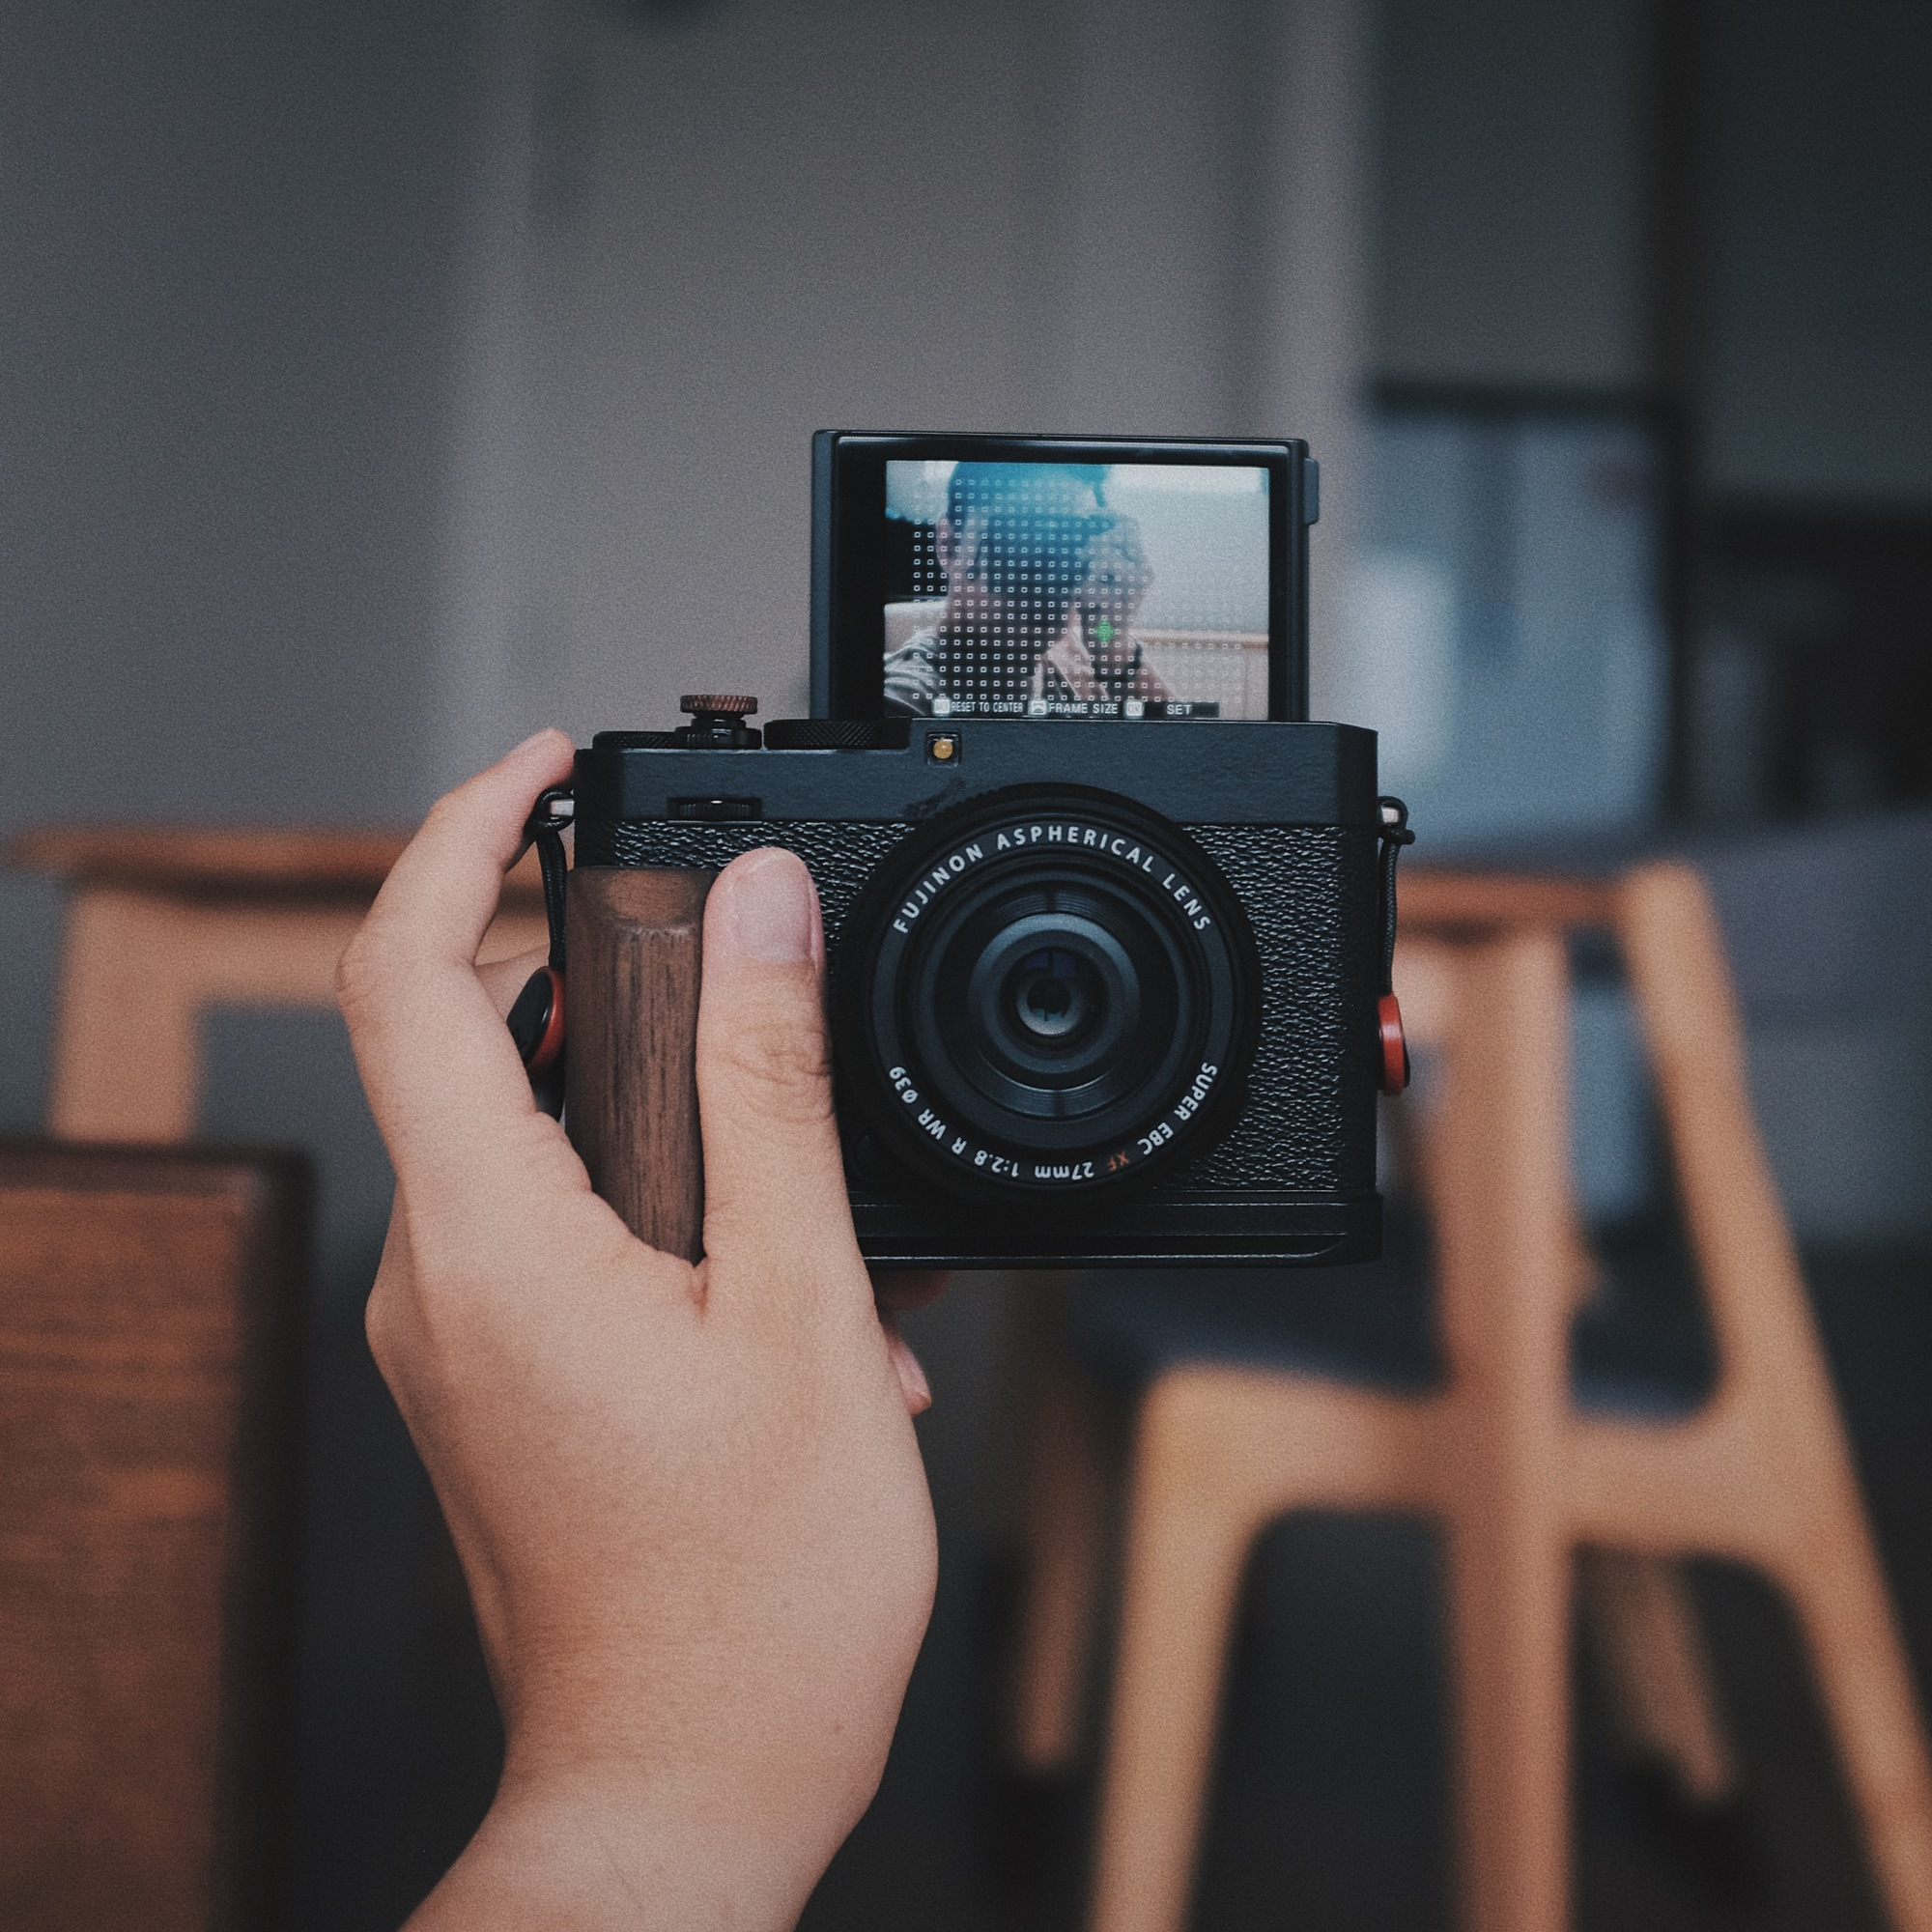
\includegraphics[width=\linewidth]{\envfinaldir/coverpic-prod.jpg}\par
            % \vskip 30pt
            \vfill

            \normalsize\rmfamily\scshape
            \copyright{} The Web Digest Project \hfill\large \envdatestr
        \end{center}
    \end{titlepage}
    % \restoregeometry
}
\newcommand{\simplehref}[1]{%
    \textcolor{blue!80!green}{\href{#1}{#1}}%
}
\renewcommand{\contentsname}{\center\Huge\sffamily\bfseries Contents\par\vskip 20pt}
\newcounter{ipartcounter}
\setcounter{ipartcounter}{0}
\newcommand{\ipart}[1]{
    % \vskip 20pt
    \clearpage
    \stepcounter{ipartcounter}
    \phantomsection
    \addcontentsline{toc}{chapter}{#1}
    % \begin{center}
    %     \Huge
    %     \sffamily\bfseries
    %     #1
    % \end{center}
    % \vskip 20pt plus 7pt
}
\newcounter{ichaptercounter}
\setcounter{ichaptercounter}{0}
\newcommand{\ichapter}[1]{
    % \vskip 20pt
    \clearpage
    \stepcounter{ichaptercounter}
    \phantomsection
    \addcontentsline{toc}{section}{\numberline{\arabic{ichaptercounter}}#1}
    \begin{center}
        \Huge
        \sffamily\bfseries
        #1
    \end{center}
    \vskip 20pt plus 7pt
}
\newcommand{\entrytitlefont}[1]{\subsection*{\raggedright\Large\sffamily\bfseries#1}}
\newcommand{\entryitemGeneric}[2]{
    % argv: title, url
    \parbox{\linewidth}{
        \entrytitlefont{#1}\par\vskip 5pt
        \footnotesize\ttfamily\mdseries
        \simplehref{#2}
    }\vskip 11pt plus 11pt minus 1pt
}
\newcommand{\entryitemGithub}[3]{
    % argv: title, url, desc
    \parbox{\linewidth}{
        \entrytitlefont{#1}\par\vskip 5pt
        \footnotesize\ttfamily\mdseries
        \simplehref{#2}\par\vskip 5pt
        \small\rmfamily\mdseries#3
    }\vskip 11pt plus 11pt minus 1pt
}
\newcommand{\entryitemAp}[3]{
    % argv: title, url, desc
    \parbox{\linewidth}{
        \entrytitlefont{#1}\par\vskip 5pt
        \footnotesize\ttfamily\mdseries
        \simplehref{#2}\par\vskip 5pt
        \small\rmfamily\mdseries#3
    }\vskip 11pt plus 11pt minus 1pt
}
\newcommand{\entryitemHackernews}[3]{
    % argv: title, hnurl, rawurl
    % \parbox{\linewidth}{
    %     \entrytitlefont{#1}\par\vskip 5pt
    %     \footnotesize\ttfamily\mdseries
    %     \simplehref{#3}\par
    %     \textcolor{black!50}{\href{#2}{#2}}
    % }\vskip 11pt plus 11pt minus 1pt
    \begin{minipage}{\linewidth}
            \entrytitlefont{#1}\par\vskip 5pt
            \footnotesize\ttfamily\mdseries
            \simplehref{#3}\par
            \textcolor{black!50}{\href{#2}{#2}}
    \end{minipage}\par\vskip 11pt plus 11pt minus 1pt
}







\begin{document}

\makeheader

\tableofcontents\clearpage




\ipart{Developers}
\ichapter{Hacker News}
\entryitemTwoLinks{Era of U.S. dollar may be winding down}{https://news.ycombinator.com/item?id=43940865}{https://news.harvard.edu/gazette/story/2025/05/era-of-u-s-dollar-may-be-winding-down/}

\entryitemTwoLinks{Man 'Disappeared' by ICE Was on El Salvador Flight Manifest, Hacked Data Shows}{https://news.ycombinator.com/item?id=43939006}{https://www.404media.co/man-disappeared-by-ice-was-on-el-salvador-flight-manifest-hacked-data-shows/}

\entryitemTwoLinks{Launch HN: Nao Labs (YC X25) – Cursor for Data}{https://news.ycombinator.com/item?id=43938607}{https://news.ycombinator.com/item?id=43938607}

\entryitemTwoLinks{Past, present, and future of Sorbet type syntax}{https://news.ycombinator.com/item?id=43938400}{https://blog.jez.io/history-of-sorbet-syntax/}

\entryitemTwoLinks{All BART trains were stopped due to `computer networking problem'}{https://news.ycombinator.com/item?id=43937242}{https://www.kqed.org/news/12039472/bart-shuts-down-entire-train-service-due-to-computer-networking-problem}

\entryitemTwoLinks{ALICE detects the conversion of lead into gold at the LHC}{https://news.ycombinator.com/item?id=43937214}{https://www.home.cern/news/news/physics/alice-detects-conversion-lead-gold-lhc}

\entryitemTwoLinks{Itter.sh – Micro-Blogging via Terminal}{https://news.ycombinator.com/item?id=43936884}{https://www.itter.sh/}

\entryitemTwoLinks{21 GB/s CSV Parsing Using SIMD on AMD 9950X}{https://news.ycombinator.com/item?id=43936592}{https://nietras.com/2025/05/09/sep-0-10-0/}

\entryitemTwoLinks{Sofie: open-source web based system for automating live TV news production}{https://news.ycombinator.com/item?id=43936408}{https://nrkno.github.io/sofie-core/}

\entryitemTwoLinks{Show HN: Aberdeen – An elegant approach to reactive UIs}{https://news.ycombinator.com/item?id=43936097}{https://aberdeenjs.org/}

\entryitemTwoLinks{NSF faces shake-up as officials abolish its 37 divisions}{https://news.ycombinator.com/item?id=43935913}{https://www.science.org/content/article/exclusive-nsf-faces-radical-shake-officials-abolish-its-37-divisions}

\entryitemTwoLinks{CryptPad: An Alternative to the Google Suite}{https://news.ycombinator.com/item?id=43935707}{https://cryptpad.org/}

\entryitemTwoLinks{Data manipulations alleged in study that paved way for Microsoft's quantum chip}{https://news.ycombinator.com/item?id=43935625}{https://www.science.org/content/article/data-manipulations-alleged-study-paved-way-microsoft-s-quantum-chip}

\entryitemTwoLinks{Amazon's Vulcan Robots Now Stow Items Faster Than Humans}{https://news.ycombinator.com/item?id=43935586}{https://spectrum.ieee.org/amazon-stowing-robots}

\entryitemTwoLinks{Implementing a Struct of Arrays}{https://news.ycombinator.com/item?id=43935434}{https://brevzin.github.io/c++/2025/05/02/soa/}

\entryitemTwoLinks{Show HN: Hyvector – A fast and modern SVG editor}{https://news.ycombinator.com/item?id=43935394}{https://www.hyvector.com}

\entryitemTwoLinks{Rust's dependencies are starting to worry me}{https://news.ycombinator.com/item?id=43935067}{https://vincents.dev/blog/rust-dependencies-scare-me/?}

\entryitemTwoLinks{WASM 2.0}{https://news.ycombinator.com/item?id=43934711}{https://www.w3.org/TR/wasm-core-2/}

\entryitemTwoLinks{Doge software engineer's computer infected by info-stealing malware}{https://news.ycombinator.com/item?id=43934540}{https://arstechnica.com/security/2025/05/doge-software-engineers-computer-infected-by-info-stealing-malware/}

\entryitemTwoLinks{The dark side of account bans}{https://news.ycombinator.com/item?id=43934313}{https://madelinemiller.dev/blog/dark-side-account-bans/}\ichapter{Phoronix}
\entryitemGeneric{\hskip 0pt{}Samsung Odyssey OLED G8 G81SF 4K UHD HDR Monitor}{https://www.phoronix.com/review/samsung-g8-g81sf}

\entryitemGeneric{\hskip 0pt{}RADV Vulkan Driver Lands BFloat16 Support In Mesa 25.2}{https://www.phoronix.com/news/RADV-Shader-BFloat16}

\entryitemGeneric{\hskip 0pt{}DeepComputing's DC-ROMA RISC-V Mainboard II For Framework Laptop Launches For \$349}{https://www.phoronix.com/news/DC-ROMA-RISC-V-Framework-Launch}

\entryitemGeneric{\hskip 0pt{}Intel NPU Linux Driver 1.17 Released}{https://www.phoronix.com/news/Intel-NPU-Linux-Driver-1.17}

\entryitemGeneric{\hskip 0pt{}Debian Looks To Better Address Ill-Maintained / Dormant Packages}{https://www.phoronix.com/news/Dormant-Debian-Packages-Issue}

\entryitemGeneric{\hskip 0pt{}Intel Xe Driver With Linux 6.16 Brings Controls For PCIe Link Downgrading On Battlemage}{https://www.phoronix.com/news/Intel-Xe-BMG-PCIe-Downgrade}

\entryitemGeneric{\hskip 0pt{}Mesa's Lavapipe Driver Wires Up More Features Used By VKD3D-Proton}{https://www.phoronix.com/news/Lavapipe-VKD3D-Proton-Features}

\entryitemGeneric{\hskip 0pt{}Hyprland 0.49 Wayland Compositor Working On Permission Management \& New Protocols}{https://www.phoronix.com/news/Hyprland-0.49-Released}

\entryitemGeneric{\hskip 0pt{}Steam Deck Adds Battery Maximum Charge Limit Control In Newest Beta}{https://www.phoronix.com/news/Steam-Deck-Max-Charge-Limit}


\ipart{Developers~~~~(zh-Hans)}
\ichapter{Solidot}
\entryitemGeneric{\hskip 0pt{}特定基因让花散发出臭味}{https://www.solidot.org/story?sid=81248}

\entryitemGeneric{\hskip 0pt{}印度要求 X 在其境内屏蔽逾 8000 个账号}{https://www.solidot.org/story?sid=81247}

\entryitemGeneric{\hskip 0pt{}罗马天主教选择首位美籍枢机为教宗}{https://www.solidot.org/story?sid=81246}

\entryitemGeneric{\hskip 0pt{}华为透露首款运行 HarmonyOS 5 的笔记本电脑}{https://www.solidot.org/story?sid=81245}

\entryitemGeneric{\hskip 0pt{}盖茨称马斯克需要为杀死最贫困儿童负责}{https://www.solidot.org/story?sid=81244}

\entryitemGeneric{\hskip 0pt{}霸王龙的直系祖先从亚洲跨越陆桥来到美洲}{https://www.solidot.org/story?sid=81243}

\entryitemGeneric{\hskip 0pt{}食用超加工食品或有害健康 }{https://www.solidot.org/story?sid=81242}

\entryitemGeneric{\hskip 0pt{}苹果高管称 Safari 上的搜索量首次下降}{https://www.solidot.org/story?sid=81241}

\entryitemGeneric{\hskip 0pt{}三分之二全球暖化是最富有 10\% 人口造成的}{https://www.solidot.org/story?sid=81240}

\entryitemGeneric{\hskip 0pt{}Gmail 停止支持 3DES 加密的传入 SMTP 连接}{https://www.solidot.org/story?sid=81239}

\entryitemGeneric{\hskip 0pt{}今天出生的人更可能遭遇极端气候事件}{https://www.solidot.org/story?sid=81238}

\entryitemGeneric{\hskip 0pt{}curl 项目遭遇 AI 生成的虚假漏洞报告攻击}{https://www.solidot.org/story?sid=81237}

\entryitemGeneric{\hskip 0pt{}特朗普政府计划修改拜登时代的 AI 芯片出口限制}{https://www.solidot.org/story?sid=81236}

\entryitemGeneric{\hskip 0pt{}人才评价机制僵化导致论文工厂屡铲不除}{https://www.solidot.org/story?sid=81235}

\entryitemGeneric{\hskip 0pt{}基因突变让部分人每天只需要睡 3 小时}{https://www.solidot.org/story?sid=81234}

\entryitemGeneric{\hskip 0pt{}欧盟制定吸引美国科学家的政策}{https://www.solidot.org/story?sid=81233}

\entryitemGeneric{\hskip 0pt{}因违反打包政策 openSUSE 移除 Deepin Desktop}{https://www.solidot.org/story?sid=81232}

\entryitemGeneric{\hskip 0pt{}绿地与新生儿的健康相关}{https://www.solidot.org/story?sid=81231}

\entryitemGeneric{\hskip 0pt{}《原神》向美国用户引入年龄验证}{https://www.solidot.org/story?sid=81230}

\entryitemGeneric{\hskip 0pt{}科学家研发出可结构重编程的磁性超材料}{https://www.solidot.org/story?sid=81229}\ichapter{V2EX}
\entryitemGeneric{\hskip 0pt{}[生活] 去年发的《孩子一同学放暑假天天来我家》后续,今天周六早晨 7 点就来报道了..}{https://www.v2ex.com/t/1130802}

\entryitemGeneric{\hskip 0pt{}[Apple] 办公室开会耳机推荐}{https://www.v2ex.com/t/1130801}

\entryitemGeneric{\hskip 0pt{}[WebRTC] 在 window 如何处理音频 aec?}{https://www.v2ex.com/t/1130800}

\entryitemGeneric{\hskip 0pt{}[程序员] 试做正则表达式解释和举例的插件}{https://www.v2ex.com/t/1130798}

\entryitemGeneric{\hskip 0pt{}[分享创造] 求评价,用 cursor 开发的 JSON 格式化网站}{https://www.v2ex.com/t/1130797}

\entryitemGeneric{\hskip 0pt{}[远程工作] 远程收 usd 还是 rmb 还是 usdt?}{https://www.v2ex.com/t/1130796}

\entryitemGeneric{\hskip 0pt{}[服务器] 感觉最近这段时间的服务器网络不是很稳定}{https://www.v2ex.com/t/1130795}

\entryitemGeneric{\hskip 0pt{}[宽带症候群] 联通连 cloudfront 都封锁了}{https://www.v2ex.com/t/1130794}

\entryitemGeneric{\hskip 0pt{}[职场话题] 今年 28,工作两年,想离开军工行业,可以跳槽去哪呢}{https://www.v2ex.com/t/1130793}

\entryitemGeneric{\hskip 0pt{}[问与答] 我觉得 claude 真的很好用,为什么不把消息限制放开?}{https://www.v2ex.com/t/1130791}

\entryitemGeneric{\hskip 0pt{}[问与答] 有人能帮我做个 rss 吗?谢谢啦!}{https://www.v2ex.com/t/1130789}

\entryitemGeneric{\hskip 0pt{}[分享创造] [AI Beauty Test] 上线了!用 AI 给你的颜值打个分,看看有啥变美小技巧?}{https://www.v2ex.com/t/1130788}

\entryitemGeneric{\hskip 0pt{}[Apple] 从旧 mac 迁移到新 mac 是否会覆盖旧的时间机器备份?}{https://www.v2ex.com/t/1130786}

\entryitemGeneric{\hskip 0pt{}[Apple] CrossOver 25 Mac 永久版 拼车 每人 124}{https://www.v2ex.com/t/1130785}

\entryitemGeneric{\hskip 0pt{}[宽带症候群] 中国移动 VIP 服务改名中国移动全球通}{https://www.v2ex.com/t/1130784}

\entryitemGeneric{\hskip 0pt{}[问与答] 家用异地组网选型}{https://www.v2ex.com/t/1130783}

\entryitemGeneric{\hskip 0pt{}[前端开发] 前端组件设计模式方面有什么可参考吗}{https://www.v2ex.com/t/1130782}

\entryitemGeneric{\hskip 0pt{}[Android] 安卓开发萌新求问}{https://www.v2ex.com/t/1130781}

\entryitemGeneric{\hskip 0pt{}[分享创造] 写了个 markdown 转知识卡片的工具 Cardify}{https://www.v2ex.com/t/1130780}

\entryitemGeneric{\hskip 0pt{}[iOS] 有没有农历生日提醒软件啊?}{https://www.v2ex.com/t/1130778}

\entryitemGeneric{\hskip 0pt{}[VPS] vps: 求推荐一些晚高峰不卡顿的 vps}{https://www.v2ex.com/t/1130777}

\entryitemGeneric{\hskip 0pt{}[生活] 愤怒!接上贴-修电瓶车记,差点摔惨!}{https://www.v2ex.com/t/1130775}

\entryitemGeneric{\hskip 0pt{}[分享创造] 下一代文本加密工具,熊曰的开源替代: Abracadabra 魔曰}{https://www.v2ex.com/t/1130773}

\entryitemGeneric{\hskip 0pt{}[问与答] 在而立之年改了名字}{https://www.v2ex.com/t/1130772}

\entryitemGeneric{\hskip 0pt{}[问与答] 有朋友还在用 Bose QC35 二代吗,最近出掉了 QC45,打算入手一个 QC35 二代}{https://www.v2ex.com/t/1130770}

\entryitemGeneric{\hskip 0pt{}[宽带症候群] 测试跨网网速的软件}{https://www.v2ex.com/t/1130768}

\entryitemGeneric{\hskip 0pt{}[问与答] 求一个 windows 后台全盘搜索方案}{https://www.v2ex.com/t/1130767}

\entryitemGeneric{\hskip 0pt{}[Apple] 当下给老妈换 iPhone ,最有性价比的选择是什么?}{https://www.v2ex.com/t/1130766}

\entryitemGeneric{\hskip 0pt{}[分享发现] Agent 哪家强?个人主观感受: Manus/扣子空间/API+MCP [附 Manus 邀请 url]}{https://www.v2ex.com/t/1130765}

\entryitemGeneric{\hskip 0pt{}[职场话题] AI 训练师是干啥的,作为一名 35+的失业前端程序员,转行做这个可行吗?}{https://www.v2ex.com/t/1130764}

\entryitemGeneric{\hskip 0pt{}[宽带症候群] 浙江电信家宽晚上 7 点以后新加坡 AWS 方向 QoS 严重}{https://www.v2ex.com/t/1130763}

\entryitemGeneric{\hskip 0pt{}[问与答] Edge 浏览器,更新频率吓人,稳定版 1 个月发布了 9 个版本?}{https://www.v2ex.com/t/1130762}

\entryitemGeneric{\hskip 0pt{}[问与答] 家里卧室没有网口,请问怎么处理?}{https://www.v2ex.com/t/1130761}

\entryitemGeneric{\hskip 0pt{}[问与答] 天天吃同事水果回点什么}{https://www.v2ex.com/t/1130758}

\entryitemGeneric{\hskip 0pt{}[全球工单系统] Windows Terminal 内存泄漏}{https://www.v2ex.com/t/1130757}

\entryitemGeneric{\hskip 0pt{}[分享创造] 我的出海 AI 服装电商产品: Coura.ai}{https://www.v2ex.com/t/1130756}

\entryitemGeneric{\hskip 0pt{}[生活] 银行推销的信用卡消费现金贷款监管严格吗}{https://www.v2ex.com/t/1130755}

\entryitemGeneric{\hskip 0pt{}[问与答] android 自动化 app 推荐}{https://www.v2ex.com/t/1130754}

\entryitemGeneric{\hskip 0pt{}[生活] 关于拍毕业照的那点破事}{https://www.v2ex.com/t/1130753}

\entryitemGeneric{\hskip 0pt{}[酷工作] [武汉] 武汉锂钠氪锶科技有限公司 Linux 研发招聘(弹性上班/周末双休/15 天春节假/五险一金/福利体检等等)}{https://www.v2ex.com/t/1130752}

\entryitemGeneric{\hskip 0pt{}[Apple] 开发了一个记账小工具,免费的哈}{https://www.v2ex.com/t/1130751}

\entryitemGeneric{\hskip 0pt{}[macOS] 野狐围棋 Mac 端做的跟屎一样}{https://www.v2ex.com/t/1130749}

\entryitemGeneric{\hskip 0pt{}[云计算] SSL 证书再有几年 47 天了,大家有什么自动化方案嘛}{https://www.v2ex.com/t/1130748}

\entryitemGeneric{\hskip 0pt{}[投资] 开通了日本富途 moomoo 证券,买点什么呢}{https://www.v2ex.com/t/1130747}

\entryitemGeneric{\hskip 0pt{}[问与答] 兄弟们,代理 IP 池业务的是厂商自己搭建还是爬取的呀?}{https://www.v2ex.com/t/1130746}

\entryitemGeneric{\hskip 0pt{}[问与答] 求推荐 Linux 桌面大语言开源客户端}{https://www.v2ex.com/t/1130745}

\entryitemGeneric{\hskip 0pt{}[Python] Python 3.14 有哪些主要更新?}{https://www.v2ex.com/t/1130744}

\entryitemGeneric{\hskip 0pt{}[程序员] 如何在 web 页面上实时预览 HTML CSS JS 效果}{https://www.v2ex.com/t/1130743}

\entryitemGeneric{\hskip 0pt{}[Android] 各位的安卓机有碰到中国移动 APP 卡首屏的情况吗}{https://www.v2ex.com/t/1130742}

\entryitemGeneric{\hskip 0pt{}[推广] 用 Cursor 打造了六款 iOS App}{https://www.v2ex.com/t/1130741}


\ipart{Generic News}







\clearpage
\leavevmode\vfill
\footnotesize

Copyright \copyright{} 2023-2025 Neruthes and other contributors.

This document is published with CC BY-NC-ND 4.0 license.

The entries listed in this newsletter may be copyrighted by their respective creators.

This newsletter is generated by the Web Digest project.

The newsletters are also delivered via Telegram channel \CJKunderline{\href{https://t.me/webdigestchannel}{https://t.me/webdigestchannel}}.\\
RSS feed is available at \CJKunderline{\href{https://webdigest.pages.dev/rss.xml}{https://webdigest.pages.dev/rss.xml}}.

This newsletter is available in PDF at
\CJKunderline{\href{https://webdigest.pages.dev/}{https://webdigest.pages.dev/}}.

The source code being used to generate this newsletter is available at\\
\CJKunderline{\href{https://github.com/neruthes/webdigest}{https://github.com/neruthes/webdigest}}.

This newsletter is also available in
\CJKunderline{\href{http://webdigest.pages.dev/readhtml/\envyear/WebDigest-20250510.html}{HTML}} and
\CJKunderline{\href{https://github.com/neruthes/webdigest/blob/master/markdown/\envyear/WebDigest-20250510.md}{Markdown}}.


\coverpic{https://unsplash.com/photos/a-temple-stands-tall-in-a-japanese-street-FbYZAV\_0VuU}{Peter Thomas}


\end{document}
